\documentclass[border=4pt]{standalone}
\usepackage{amsmath,amssymb,amsfonts}
\usepackage{xcolor,colortbl,array,booktabs,multirow}
\usepackage{tikz}
\usepackage{pgfplots}
\pgfplotsset{compat=1.16}
\usetikzlibrary{arrows, automata, backgrounds, calendar, chains, decorations,
    matrix, mindmap, patterns, petri, positioning, shadows, shapes.geometric,
    trees, shapes, decorations.pathreplacing, calc, tikzmark, arrows.meta,
    intersections, fit, graphs, quotes, angles, decorations.markings}
\newcommand{\st}{\text{ s.t. }}
\newcommand{\x}{\mathbf{x}}
\renewcommand{\b}{\mathbf{b}}
\renewcommand{\c}{\mathbf{c}}
\newcommand{\A}{\mathbf{A}}
\newcommand{\y}{\mathbf{y}}
\newcommand{\z}{\mathbf{z}}
\newcommand{\R}{\mathbb{R}}
\newcommand{\RR}{\mathbb{R}}
\newcommand{\Z}{\mathbb{Z}}
\newcommand{\ZZ}{\mathbb{Z}}
\newcommand{\npcomplete}{NP-complete}
\providecommand{\true}{\text{TRUE}}
\providecommand{\false}{\text{FALSE}}
\tikzset{vertex/.style={circle,fill=black!25,minimum size=20pt,inner sep=0pt},
    edge/.style={draw,thick,-},weight/.style={font=\small},
    selected vertex/.style={vertex, fill=red!24},
    selected edge/.style={draw,line width=2pt,-,red!50},
    ignored edge/.style={draw,line width=2pt,-,black!20}}
\newcommand{\vect}{\vec}
\providecommand{\ds}{\displaystyle}
\providecommand{\longvect}{\overrightarrow}
\usepackage[normalem]{ulem}
\definecolor{ocre}{RGB}{243,102,25}
\providecommand{\leftB}{\left[}
\providecommand{\rightB}{\right]}
\tikzset{directed/.style={postaction={decorate,decoration={markings,mark=at position .65 with {\arrow{>}}}}},
    directed1/.style={postaction={decorate,decoration={markings,mark=at position .65 with {\arrow{>}}}}}}
\begin{document}
\begin{tikzpicture}[remember picture, overlay, >=stealth]

% Green arrow: Final objective
\draw[->, thick, green!60!black] 
  ($(pic cs:zstart2)+(0,0.1)$) -- ++(-2.5,1.0) node[left, green!50!black] {Final objective: $z = 23$};

% Yellow arrows: Basic variables
\draw[->, thick, blue] 
  ($(pic cs:x2)+(-0.2,-0.2)$) -- ++(-3.0,-0.5) node[left, blue] {Basic var: $x = 4$};
\draw[->, thick, blue] 
  ($(pic cs:y2)+(-0.2,-0.2)$) -- ++(-3.0,-0.5) node[left, blue] {Basic var: $y = 5$};
\draw[->, thick, blue] 
  ($(pic cs:s22)+(-0.2,-0.2)$) -- ++(-3.0,-0.5) node[left, blue] {Basic var: $s_2 = 3$};

% Red arrows: Non-basic variables
\draw[->, thick, red] 
  ($(pic cs:zend2)+(0.2,0.3)$) -- ++(1.2,1.0) node[right, red] {Non-basic: $s_1 = 0$};
\draw[->, thick, red] 
  ($(pic cs:zend2)+(0.4,0.1)$) -- ++(1.5,0.5) node[right, red] {Non-basic: $s_3 = 0$};

\end{tikzpicture}
\end{document}
